\chapter{Introduction}
\label{chapter1}

\section{Gravitational Waves}

Almost all of humanity's knowledge of the universe is derived from
observations of electromagnetic waves.  The effort to detect
gravitational waves seeks to expand this knowledge by observing an
entirely different field, and to further verify the correctness of the
theory of general relativity.

Any theory of gravity that avoids instantaneous action at a distance
must feature some kind of gravitational waves.  Even Newtonian gravity
can be modified to account for propagation delays from massive bodies
that are the sources of attraction\cite{Schutz1984Gravitational}.
Gravity as we know it, however, is described by the general theory of
relativity.  In general relativity, spacetime is treated as a
four-dimensional manifold with some intrinsic curvature.  This
curvature is generated by the presence of mass and energy.  In the
absence of forces, particles follow geodesic trajectories on this
manifold.  Quintessentially, ``Space tells matter how to move; matter
tells space how to curve''~\cite{MTW}.

This relationship between matter and curvature is made formal through
the Einstein field equation, which equates (up to units) the Einstein
tensor ($\mathsf{G}$), encoding curvature, with the
Stress-Energy tensor ($\mathsf{T}$), encoding the matter and energy
contents:
\begin{equation}
\mathsf{G} = \frac {8\pi G}{c^4} \mathsf{T}
\end{equation}
where $G$ is (Newton's) universal gravitational constant and $c$ is
the speed of light.

To perform calculations, we typically need to work in some coordinate
basis.  Thus one will work with $G_{\mu\nu}$, where $\mu$ and $\nu \in
{0,1,2,3}$ are coordinate indices.  In this notation, the Einstein
tensor is given by $G_{\mu\nu} = R_{\mu\nu} - \frac{1}{2} R
g_{\mu\nu}$, where $R_{\mu\nu}$ is the Ricci curvature tensor, $R$ is
the Ricci scalar, and $g_{\mu\nu}$ is the spacetime metric.  The
metric plays a central role here, as it both encodes the curvature and
implicitly defines the coordinate system.

To reveal the mechanism of gravitational waves, we are interested in
vacuum ($\mathsf{T}=0$) solutions of the Einstein field equations in
the weak-field limit.  In the weak-field limit, we can write the
metric $g_{\mu\nu}$ as the sum of the flat-space Minkowski metric
$\eta_{\mu\nu}$ and a small perturbation $h_{\mu\nu}$:
$$g_{\mu\nu} = \eta_{\mu\nu} + h_{\mu\nu}$$ This is the regime of
linearized gravity.  Calculating out the Einstein field equation
keeping only terms of first-order in $h$ and choosing the
transverse-traceless gauge, one finds\cite{Carroll1997Lecture} a wave
equation for $h$:
$$\left(\nabla^2 - \frac{1}{c^2}\frac{\partial^2}{\partial t^2}\right)h_{\mu\nu} = 0$$
where $h_{\mu\nu}$ has, for a wave propagating along the $z$ axis, the form:
$$ [\mathsf{h}(z,t)] = \left(
\begin{array}{cccc}
0 & 0       &  0      & 0 \\
0 & h_+     &  h_\times & 0 \\
0 & h_\times & -h_+     & 0 \\ 
0 & 0       &  0      & 0 
\end{array}
 \right) \cos\left(2\pi f (t - z/c)\right)
$$
Here we see several of the essential points of gravitational waves:
\begin{itemize}
\item There are two independent components (polarizations)
\item They travel at the speed of light 
\item They are manifest as a transverse tidal force on inertial objects
\end{itemize}

In the transverse traceless gauge, inertial objects reside at fixed
coordinates.  To see the effect of a gravitational wave, suppose
inertial test masses reside at coordinates $0$ and $L_0$ along the $x$
axis, and suppose a gravitational wave is incident along the $z$ axis.
The proper length between two points is given by
\[
L = \int \sqrt{-g_{\mu\nu} dx^\mu dx^\nu}
\]
Integrating along the $x$ axis, and assuming that the metric takes
the form $g = \eta + h$, we find
\begin{align}
L & = \int \sqrt{g_{xx}} dx \\
%  = \int \sqrt{1 + h_+} dx
  & = L_0 \sqrt{1 + h_+} \\
  & \approx L_0 \left(1 + \frac{1}{2} h_+\right).
\end{align}
\begin{figure}
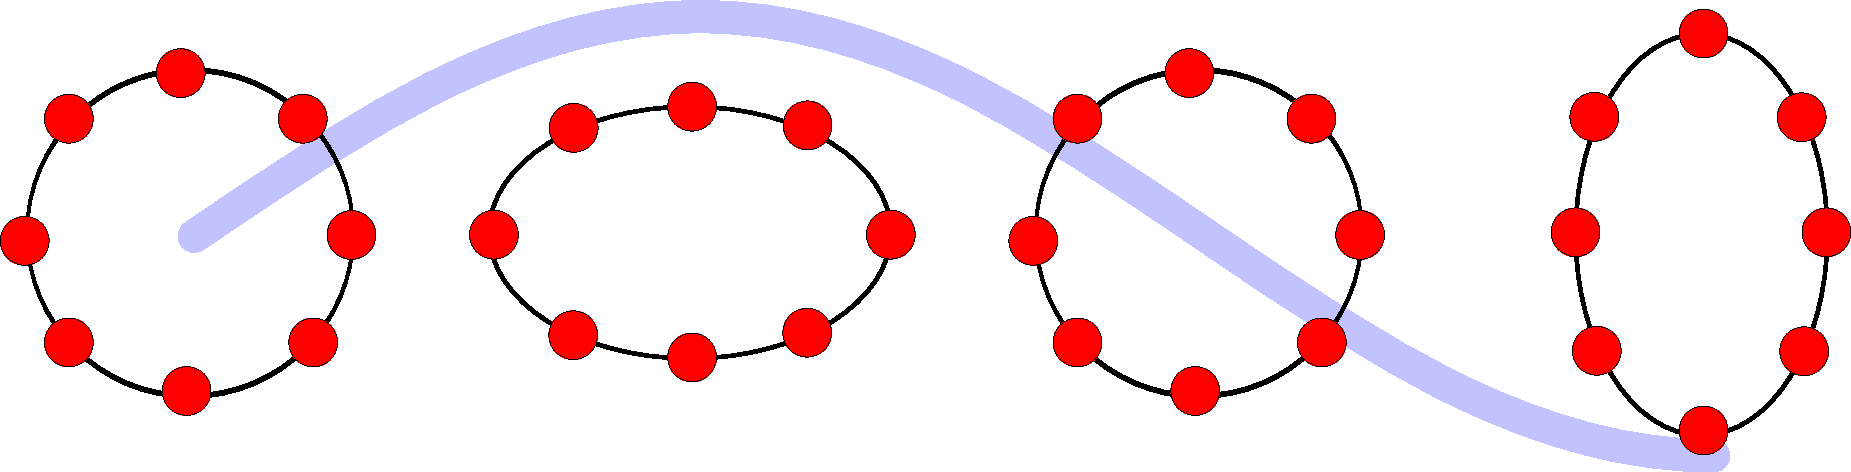
\includegraphics[width=\columnwidth]{chapter1/figures/gwave.pdf}
\caption[Effect of a gravitational wave on a ring of test
  particles]{\label{fig:gwave-effect}Effect of a gravitational wave
  (traveling into or out of the page) on a ring of non-interacting
  inertial test particles, with the gravitational wave waveform 
  superimposed.}
\end{figure}
The gravitational wave lengthens the path by $\Delta L =
\frac{1}{2}h_+$. Half a period later, the wave will shorten the path
length by the same amount.  Simultaneously, a similar path along the
$y$ axis will see a $\Delta L$ of the opposite sign.  This oscillatory
transverse stretching and compressing is depicted in
figure~\ref{fig:gwave-effect}.  Because the change in optical path
length has the form of a change in length per unit length, it is often
described as a \emph{strain}.

A photon traveling from one test mass to another will see this change
in proper length, assuming that the gravitational wave phase (and thus
the metric) changes negligibly in the time required by the photon to
make the trip.  This is the basis of laser interferometric
gravitational wave detectors: if we can arrange mirrors as inertial
test masses, then we can imprint the gravitational wave onto the phase
of laser light.

\section{Generation of gravitational waves}

Conservation of energy and momentum forbid changes in the monopole and
dipole moments of an isolated mass distribution.  The leading
multipole term leading to gravitational wave radiation is therefore
the quadrupole moment, which is forbidden by no conservation law.  For
instance, two objects in orbit around one another exhibit a
time-varying quadrupole moment.

%% The gravitational radiation generated by an accelerating quadrupole
%% moment is\cite{Saulson1994Fundamentals}
%% %
%% \[
%% h_{\mu\nu} = \frac{2 G}{r c^4} \ddot{I}_{\mu\nu}(t-r/c)
%% \]
%% where $r$ is the distance from the source, $I$ is the quadrupole
%% moment, and $\ddot{I}$ is its second derivative.

A typical GW source of interest is a pair of massive objects revolving
around their common center of mass in a binary orbit.
Maggiore\cite{Maggiore2008Gravitational} gives the strain in the two
polarizations $h_+$ and $h_\times$ due to two objects in a circular,
binary orbit as
%
\begin{align}
h_+(t)     &= \frac{4}{r} \frac{G \mu \omega^2 R^2}{c^4} \frac{1}{2} (1 + \cos(\theta)^2)  \cos (2 \omega t) \\
h_\times(t) &= \frac{4}{r} \frac{G \mu \omega^2 R^2}{c^4} \cos(\theta) \sin (2 \omega t)
\end{align}
where $r$ is the distance to source, $\mu$ is the reduced mass of the
binary system, $R$ is the radius of the binary orbit, $\theta$ is the
angle between the normal of the orbital plane and the line of sight to
the observer, and $2 \omega$ is the gravitational wave frequency. Some
points to note include:
\begin{itemize}
\item The gravitational wave strain drops only with $1/r$ with distance
  from the source, in contrast to the inverse square law by which
  electromagnetic observations suffer.
\item The gravitational wave frequency is twice the orbital frequency.
\item The emission is surprisingly isotropic.
\item Most of the GW emission is along the rotational axis of the
  binary system; these GW's are circularly polarized.  Emission in the
  plane of the binary system is linearly polarized.  This is as one
  would expect from basic symmetry considerations.
\end{itemize}

To get a sense of the scale of the phenomenon, we can plug in some
numbers.  A binary system in the Virgo cluster orbitting at 50 Hz
where each object is a one-solar-mass star would produce an expected
strain on earth of the order $h\sim10^{-21}$-- an almost
preposterously small effect, making GW detection a significant
challenge.

\begin{comment}
r = 5e23;
mu = 1e30;
G = 5.574e-11;  % N m^2 / kg^2
c = 299792458;  % m / s
f = 100;        % Hz
omega = 2*pi * f;
R = ((2 * mu)/(G * omega^2))^(1/3);
h = (4/r) G * mu * omega^2 * R^2 / c^4;
\end{comment}
\begin{comment}
\begin{align}
r   &= 16 \text{ MPc} \approx 5 \times 10^{23} \text{ m} \\
\mu & = (1/2) m_\odot \approx  1 \times 10^{30} \text{ kg} \\
R   & = \left(2 \mu / (G \omega^2)\right)^{1/3}
\end{align}
\end{comment}
\section{The Hulse-Taylor Pulsar}

The emission of gravitational waves by a binary star system has
already been confirmed--indirectly.  In 1974, Hulse and Taylor
discovered a radio pulsar that is a member of a binary star
system\cite{Hulse1975Discovery,Weisberg2005Relativistic}.  The
electromagnetic emissions of the pulsar allowed the orbital parameters
of the binary system to be precisely tracked over a long period of
time.  As the system spins, energy is radiated away from the orbital
system in the form of gravitational waves. Measurement of the orbital
period through pulsar tracking over 30 years shows that the orbit is
decaying exactly as predicted by general relativity.

Another binary system containing pulsars was discovered in 2004.  In
this system \emph{both} objects are
pulsars\cite{Lyne2004DoublePulsar,Kramer2006Tests}.

\section{Detectors}
%Gravitational waves couple to both light and matter.

\begin{figure}
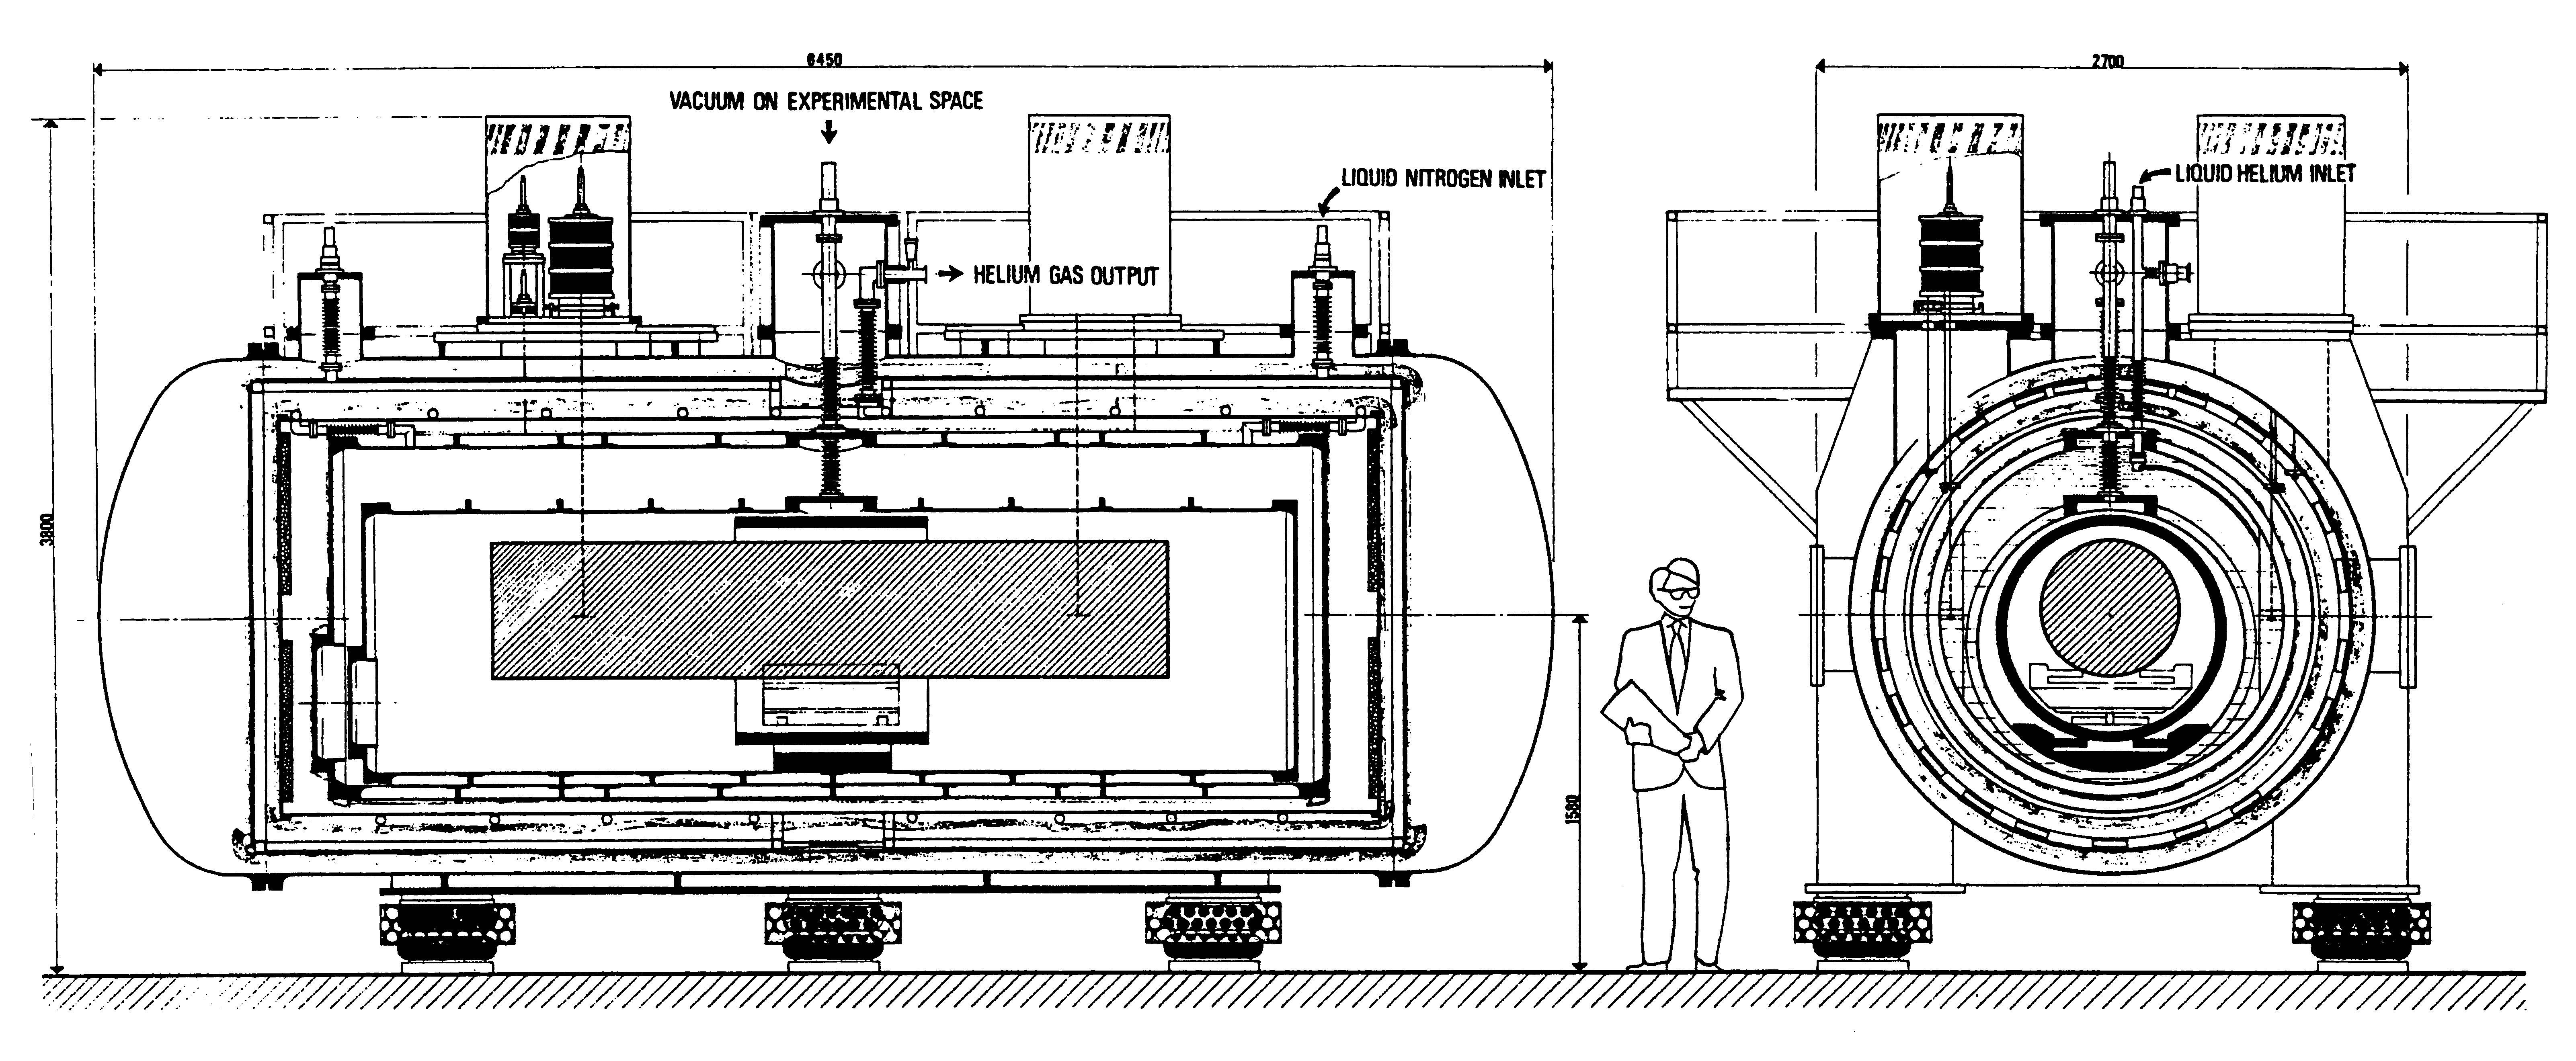
\includegraphics[width=\columnwidth]{chapter1/figures/explorer.png}
\caption[EXPLORER bar detector]{\label{fig:explorer-bar}Depiction of
  the cryostat of the {\sc explorer} bar detector, which has operated
  at {\sc cern} since 1990.  {\sc Explorer} was oriented in parallel
  to the {\sc allegro} detector at LSU\cite{Mauceli1996Allegro} to
  enable searches for coincident detections.  Illustration adapted
  from~\cite{Astone1993Longterm}.}
\end{figure}

The first attempts to detect gravitational waves used resonant bar
detectors\cite{Thorne1980Gravitationalwave,Levine2004Early}.  
In such a detector, a large cylinder of a metal alloy with
a very high mechanical Q-factor is suspended in a vacuum chamber and
cooled to cryogenic temperatures.  A passing gravitational wave
couples mechanical energy into the bar, ringing up the fundamental
mechanical mode of the bar.  Sensitive detectors (latter bars used
SQUIDs) read out this mechanical displacement.  Resonant bars are
inherently narrow-band devices, sensitive to gravitational waves
within a narrow linewidth about their fundamental resonance.

Bar detectors do have the advantage that they are small enough that
they can be moved or re-oriented.  The ALLEGRO bar detector at LSU~\cite{Mauceli1996Allegro} was
rotated to modulate its overlap function with the nearby LIGO
Livingston observatory.%\cite{Abbott2007First}

\subsection{Laser interferometers}

Inaugurated by an initial study by Rai
Weiss\cite{Weiss1972Electromagnetically} and experiments by Robert
Forward\cite{Forward1978Wideband} in the 1970's, 
laser interferometers are now the instrument of choice in the search
for gravitational waves.  A gravitational wave will modulate the
optical path length of light traveling between inertial test masses.
This path length modulation can be detected by a laser interferometer.
%
In terrestrial interferometers, large ($\sim10$kg) glass cylinders
serve as both super-polished mirrors and inertial test masses.  These
optics are hung as pendula to allow inertial freedom of the pendular
resonance frequency and enclosed in a large, high-vacuum enclosure.

Large laser-interferometer gravitational wave detector installations
include LIGO\cite{S5InstrumentPaper} in the United States,
VIRGO\cite{Acernese2008Virgo} in Italy, and GEO600\cite{GeoStatus2008}
in Germany.
%
The operation of laser interferometer gravitational wave detectors is
the focus of this work and is detailed in the following chapters.

\subsection{Other detectors}

There are a few other mechanisms by which gravitational waves may be
detected, or by which their influence may be observed.

Pulsars serve as extremely reliable clocks, beaming a sequence of
pulses towards earth whose arrival times can typically be predicted to
better than a microsecond.  The path of the electromagnetic waves
traveling from the pulsar to earth acts in some ways like an arm of a
laser interferometer: gravitational waves passing transversely to the
Earth-Pulsar baseline will modulate the optical path length, producing
perturbations in the arrival time of the pulsar pulses--perturbations
which are correlated between observations of distinct pulsars. Pulsar
timing arrays seek to analyze these correlated residuals to find
evidence of gravitational waves;
Hobbs~\cite{Hobbs2009International} anticipates that pulsar timing
analysis will yield detections of gravitational waves in the nanohertz
regime (period 3-30 years) in the next 5-10 years.

Primordial gravitational waves will also leave their imprint on the
polarization of the cosmic microwave background radiation.  Many CMB
polarization experiments are currently underway
(e.g.~\cite{Filippini2011SPIDER}), searching for the faint ``B-modes''
in the microwave polarization.

\subsection{Detector products}

The data produced by a gravitational wave detector consist of the
calibrated strain time series $h(t)$ (current detectors are sensitive
to only a single polarization) along with auxiliary data streams which
convey the state of the detector and its environment.  These auxiliary
data streams are used for both detector debugging and for vetoing of
candidate signals which are coincident with local environmental
disturbances.

\section{Sources of Gravitational Waves}
Anticipated sources of gravitational waves can be conveniently
categorized as \emph{continuous} or \emph{transient}, and as
\emph{modeled} or \emph{unmodeled}.  There is some overlap in this
division.  Associated with each potential source of gravitational
waves are \emph{search efforts} which search the data produced by
extant gravitational wave detectors for evidence of GWs from that 
source.

\begin{itemize}

\item \textbf{compact binary coalescence} --- Pairs of compact objects
  (black holes or neutron stars) in binary orbits are expected to lose
  energy through gravitational waves, causing the orbit to decay until
  the objects finally begin to interact and merge into a single
  object.  This inspiral process will generate a characteristic chirp
  signal, followed by the complex merger process and then ringdown.

\item \textbf{continuous wave} --- Rapidly spinning objects will
  generate essentially monochromatic signals, which are in turn
  doppler-shifted by the relative motion of the Earth and the source.
  The search for these signals is sometimes called the pulsar search, since the primary source
  in this category is expected to be rapidly spinning neutron stars
  (such as pulsars).  The search, in turn, is divided into searches
  for known pulsars and unknown pulsars.  Pulsars which are known
  electromagnetically can be targetted directly, whereas unknown
  pulsars require a brute-force search of the parameter space.

  Currently this is attacked in part through the distributed computing
  project Einstein@Home.  Interestingly, the pulsar search 
  works equally well for analyzing radio telescope data; 
  several previously
  unknown radio pulsars have been discovered by feeding Aricebo data
  into the Einstein@home project\cite{Knispel2010Pulsar}.  

\item \textbf{bursts} --- Transient cataclysmic events such as
  supernovae will generate bursts of gravitational waves whose
  waveforms is not known in advance.  

\item \textbf{stochastic background} --- In the same manner as the
  cosmic microwave background radiation, a cosmological background of
  gravitational waves is expected to exist.  This is perhaps the most
  exotic anticipated source of gravitational waves, since its
  detection will inform us of the state of the universe at an age far
  earlier than has yet been probed.  Sadly, the cosmological
  background is almost certainly too weak to detect in the forseeable
  future.

  The cacophony of unresolved astrophysical sources will also combine
  to produce a gravitational wave stochastic background.   

  The stochastic background search is fully coherent.  In its simplest
  form, the search simply computes the correlation between pairs of
  gravitational wave detectors.  This can be done in either an all-sky
  search or in a sky-position-dependent search.  Typically, some
  power-law gravitational wave spectrum is assumed.
  
  The signal processing strategy for the detection of a stochastic background
  is described by Allen and Romano in \cite{Allen1999Detecting}.
\end{itemize}

Improvements in search sensitivity can be achieved by incorporating
knowledge of the expected signal waveform or spectrum; integrating
over a long period of time (for continuous sources); and by looking
for coincidence or coherence between multiple detectors.

The global network of gravitational wave detectors is operated as a
sensor array, an interferometer composed of many interferometers.

\section{LIGO}

Ground was broken on the first of the two LIGO observatories in 1994.
After years of construction and then detector commissioning, the three
detectors at the two observatories reached their design sensitivity\cite{LigoSRD} in
2004\cite{Ballmer2006LIGO}.  Having reached this milestone, the attention turned to
collecting data for astrophysical observation rather than instrument
development.  By October 2007, the LIGO project accomplished the goals
of what is now known as ``initial LIGO,'' having collected 1 year of
observational data with all three detectors online simultaneously, over
the course of the 5th science run (known as S5).

It had always been intended that this initial generation of LIGO would
be followed by a programme of improvements\cite{Abramovici1992LIGO}.  The next generation of
LIGO detectors is ``Advanced LIGO,'' which will feature significantly
more effective (and more complex) seismic isolation, an increase of
$20\times$ in laser power, in addition to other improvements.

Rather than spend the entire time before the onset of Advanced LIGO
taking observational data in the Initial LIGO configuration, it was
decided to implement an intermediate series of upgrades in a project
that came to be called ``Enhanced
LIGO''\cite{Adhikari2006Enhanced,T050252,JoshSmithEnhancedAdvanced}.
The goals of enhanced LIGO were to both increase the chances of an
early discovery (by increasing the detector sensitivity), and to gain
early experience with Advanced LIGO technologies.

The observational data collected so far has been analyzed (and
continues to be analyzed) for evidence of gravitational waves.
Although no gravitational waves have yet been detected, these searches
have set the tightest upper limits to date on GW emission.  Results of
searches for compact binary inspirals\cite{S5CBCnospin, S5CBC5months},
unmodeled bursts\cite{S5burst}, known pulsars\cite{S5knownpulsars},
GWs associated with a gamma-ray burst\cite{S5GRB070201},
and the stochastic backround\cite{S5NatureStochastic} have recently
been published.

\subsection{Summary of changes made for Enhanced LIGO}

% FIXME Gaby says: You need a better description of initial
% detectors' technology so that the next section makes sense.  

Detector upgrades during Enhanced LIGO included:
\begin{itemize}
\item An increase in laser power.  The initial LIGO laser, an Nd:YAG
  NPRO capable of producing $< 10$ Watts of laser power at a
  wavelength of 1064 nm, was replaced with the Advanced LIGO laser
  front-end, built by Laser-Zentrum Hannover, with an output power of 35 W.
\item The input optics were redesigned to handle the higher input
  power~\cite{DooleyCharacterization,Quetschke2008ElectroOptic}.  
\item A new thermal compensation system was implemented to compensate
  for the greater amount of thermal lensing that would be induced by
  the higher operating power.
\item An output mode cleaner was installed, supported by a prototype
  of the advanced LIGO in-vacuum seismic isolation system~\cite{KisselThesis}
\item The Angular Sensing and Control system was redesigned to cope
  with angular instabilities introduced at high
  power~\cite{Sidles2006Optical,DooleyAngular}
\item Readout of the gravitational wave channel was changed from RF
  readout to DC readout.
\end{itemize}

% \cite{StatusS5} ?
The state of the LIGO detectors before these modifications is
described in \cite{S5InstrumentPaper} as well as numerous PhD
dissertations, notably Rana Adhikari's \cite{RanaThesis} and and
Stefan Ballmer's \cite{Ballmer2006LIGO}.  Robert Ward's dissertation
details the implementation and evaluation of DC readout at the LIGO 40
meter prototype interferometer in Pasadena \cite{RobWardThesis}.
%
During the same time as Enhanced LIGO, DC readout was simultaneously
and independently implemented at GEO\cite{GeoDC,Degallaix2010Commissioning}.

\section{The Future}

It is hoped that Advanced LIGO and Advanced VIRGO, currently under
construction, will bring the first direct detection of gravitational
waves and begin the era of regular detection and gravitational wave
astronomy.
%
Beyond the `Advanced' detectors, several next-generation
interferometers are also in the works.

Technological development of terrestrial laser
interferometers is a vibrant field.  The Advanced detectors are
anticipated to be limited almost everywhere by quantum mechanical
noises, making gravitational wave detectors a verdant field for work
in quantum optics.  The next generation of terrestrial gravitational
wave detectors will be limited by near-field gravity--``Newtonian
noise'' from density waves in the surrounding environment.  The ways
forward will be to move underground (where this effect is smaller);
measure, predict, and subtract the Newtonian noise contribution using
a seismic sensor array; or to move into space.
%
The Einstein telescope~\cite{EinsteinTelescopeDesignStudy2011} is a
proposed syst of three interferometers with arms forming an
equilateral triangle, to be installed in tunnels deep under Europe.

Going into space makes feasible the use of extraordinarily long arms
and yields complete freedom from terrestrial noise, allowing access to
very low frequency gravitational waves.  The Laser Interferometer
Space Antenna (LISA) design is composed of three spacecraft forming an
equilateral triangle, the whole constellation in solar orbit.  These
spacecraft will house truly inertial test-masses, floating within an
internal vacuum enclosure while external microthrusters keep the
spacecraft centered around the test mass, a configuration known as a drag-free satellite~\cite{Lange1964DragFree}.  The gravitational wave
channel is derived using time-delay interferometery.  The proposed
LISA design is sensitive to gravitational waves in the range $10^{-4}$
to $10^{-1}$ Hz (period of 3 hours down to 10 seconds).

\section{This Dissertation}
% FIXME Gaby says: You need to introduce the LIGO project as
% NSF-funded, and the LIGO Scientific Collaboration of which yu are a
% member. You should also say that although the work is done in
% general in collaboration with many other LSC members, you have made
% unique contributions and measurements that will be highlighted in
% the thesis.

This dissertation describes the implementation of DC readout and an
output mode cleaner during Enhanced LIGO.

In Chapter 2, I explain the principles and practice behind the
sensitivity of the LIGO detectors.  I show how the machine converts
gravitational wave-induced phase modulation into a modulated optical
field while offering a large amount of immunity to other effects.

In Chapter 3, I describe DC readout.

Chapter 4 introduces the Output Mode Cleaner, its design and control,
and the general idea of mode cleaners.

Finally, in Chapter 5, I present results demonstrating the performance
of this system.

%Additional references to cite: \cite{Garfinkle2005Gauge,
%  Heinzel1999Advanced,Saulson1994Fundamentals,
%  Harris1996Gravitational,Melissinos2010Response}.

\section{Acknowledgement}

This work was supported by the National Science Foundation under grant
\href{http://www.nsf.gov/awardsearch/showAward.do?AwardNumber=0905184}{PHY-0905184}.
LIGO was constructed by the California Institute of Technology and
Massachusetts Institute of Technology with funding from the National
Science Foundation and operates under cooperative agreement
\href{http://www.nsf.gov/awardsearch/showAward.do?AwardNumber=0757058}{PHY-0757058}.
This dissertation has LIGO Document number LIGO-P1000010.
